\chapter{The effect of Rossby number dependent latitudinal differential rotation on the observed rotation period distribution}
\label{chap:period_gap}

Portions of the content of this Chapter will form an upcoming published work.

\section*{Abstract}

Photometric variability due to stellar spots allows astronomers to measure the surface rotation periods of stars.
Within multiple missions' rotation period samples (e.g. \kepler, \ktoo, \ZTF), there is a distinct dearth of observations of stars rotating at intermediate periods 15 $\gtrsim P_{rot} \gtrsim$ 20 days.
This dearth of observations is known as the intermediate period gap.
The position of this gap varies with the colour of the stars.
Various mechanisms have been proposed to explain the dearth of observations from stars physically \update{``jumping"} the gap through enhanced wind-braking, to stars above and below the gap representing two populations of stars, to the gap representing a minimum probability of observing rotation periods.
The exact cause of the \update{gap} is currently unknown.
In this Chapter, we propose the hypothesis that the gap represents a sudden increase in the observed rotation period of stars through the onset of equator-fast latitudinal differential rotation.
The rotation period gap can be reproduced under this mechanism with observationally derived relations between equatorial and differential rotation evolution.

\newpage

\section{Introduction}
\label{sec:intro}

Measurement of the rotation period of samples of stars allows us to understand internal mechanisms that we otherwise would not be able to probe.
%%For example, the mass-dependent core-envelope coupling and decoupling of young stars have only recently been observed by measuring the rotation period of stars with age through the rotation period distribution of clusters \citep{reinhold_rotation_2015-1}.
%An unexplained feature of the rotation period distribution of low-mass main-sequence stars comes in the form of what is known as the intermediate period gap.
The intermediate period gap represents a minimum of observations of stars with particular rotation periods measured from photometric variability due to stellar spots first observed by \citet{mcquillan_rotation_2014}.
The intermediate period gap is robust between different photometric observation missions \citep{mcquillan_rotation_2014,davenport_rotating_2017,davenport_rotating_2018,lu_bridging_2022} and multiple period detection methods applied to these missions.

The rotation period here is inferred from periodic variations in the brightness of stars from active regions coming in and out of the observer's line of sight from the rotation of its surface.
It is unknown whether the intermediate period gap occurs in other techniques to measure the rotation of stars; if it does, it would allow us to focus on particular explanations for the gap.
Rotational splittings of low-mass stars, where the gap is most apparent, have not been observed, and it is currently unknown whether the intermediate period gap is also a feature observed in spectroscopic observations of surface rotation velocity.
While spectroscopic surface velocity has been measured for orders of magnitude more stars than surface rotation periods from stellar spots have, the inclination angle effect, as only \vsini\ can be measured, and uncertainties in stellar radius would smear out decreased densities of observations.
Direct observation of the intermediate period gap from spectroscopic surface velocity has not been made.

The position of the gap varies in period with respect to mass. 
The quality cuts made to data sets in which rotation period is attempted to be measured \citep[e.g., removing binaries and subgiants as in the analysis of ][]{mcquillan_rotation_2014, claytor_tess_2023} are not biased away from detecting stars within the gap.
%If the gap aligned itself with a line of constant rotation in only one mission, then the mechanism underlying the gap could be more readily explained through the selection function of said mission.
These factors suggest that the intermediate period gap represents a function of stellar evolution or an unaccounted-for problem in observing rotation periods through photometric oscillations from stellar spots.

%leading the reader.
The intermediate period gap is characterised by a number of features as shown in Figure \ref{fig:big_prawn}.
The density of stars above and below the gap is roughly constant; the density of observations drops swiftly in the gap.
The gap also aligns with a line of constant Rossby number, suggesting a common phase evolution rather than age.
This is interesting because photometric variability drops toward the gap from below and above, suggesting a common phase of magnetic evolution.
We also observe that the dearth is most apparent for lower mass (\teff\ $<$ 4500 K) stars.
While not shown in this plot, they are nonetheless indicative of the nature of the gap: the intermediate period gap disappears for fully convective stars \citep{lu_bridging_2022}.
Stars above and below the gap are also not significantly observationally distinct except in the rotation period.
Further, \citet{lu_bridging_2022} argued that stars above and below the gap are of similar kinematic age.
An explanation for the gap must explain all of these features.

\begin{figure}
\centering
 \includegraphics[width=\textwidth]{Figures/rot_gap_figures/big_prawn.png}
 \caption[The rotation period distribution of the \citep{mcquillan_rotation_2014} sample highlighting the features of the intermediate period gap.]{The rotation period distribution of the \citep{mcquillan_rotation_2014} sample highlighting the features of the intermediate period gap. \textbf{Top:} A 2D histogram of the logarithm of the rotation period against the effective temperature of the rotation period sample coloured by the number of stars in each bin ($N$). Here, we observe the dearth of observations of rotation period for stars with \teff \ $<$ 5000 (K) between $\log_{10} \ P_{\rm{rot}}\ / \ d$ = 1 and 1.5, increasing in $P_{\rm{rot}}$ as \teff \ decreases: the intermediate period gap. \textbf{Bottom:} The logarithm of the rotation period against the effective temperature of the rotation period sample coloured by the logarithm of \rper{}. The alignment of the minimum in \rper\ and the position of the intermediate period gap is also highlighted here.  
 \textbf{Top inset:} a histogram of the logarithm of the rotation period for stars with 4000 $<$ \teff \ (K) $<$ 4200. Here, we observe the dearth of observations of stars in this effective temperature range occurs at $\sim \ \log_{10} \ P_{\rm{rot}}\ / \ d \ = 1.2$. 
 \textbf{Bottom inset:} The logarithm of the rotation period against the logarithm of \rper \ for stars with 4000 $<$ \teff \ (K) $<$ 4200. Comparing the two inset plots, it is clear that the intermediate period gap and the decrease in \rper \ align with the same position in regards to the period and effective temperature.}
 \label{fig:big_prawn}
\end{figure}


Multiple mechanisms have been proposed to explain the intermediate period gap.
\citet{mcquillan_rotation_2014} first proposed that the gap represents bimodal bursty star formation in the local \kepler{} field.
They suggest that the lower rotation period (faster rotators) prong represents a younger population, and the upper rotation period prong represents an older population, with the gap representing a minimum in star formation at a particular time.
\citet{davenport_rotating_2018} support local bursty star formation hypothesis by separating the \kepler{} rotation period distribution by distance through \gaia{} \ parallaxes.
They find that the gap appears to disappear for stars further away than 525 pc.
At those distances, observations of stars are magnitude-limited to brighter high-mass stars (M $\geq$ 0.9 M$_{\odot}$), where observations of the gap are tentative and period detection is much less precise.
If the gap extends up to these high-mass stars, then its existence can be blurred out by the imprecision of these measurements.
Their work may also support this explanation.
In the full \citep{mcquillan_rotation_2014} sample the gap disappears for high mass ($M \ \geq \ 0.8 M_{\odot}$, $B_P - R_P \ \leq \ 1.0$) stars.
In the distance limited ($\leq$ 525pc) sample, the gap appears to permeate to these higher-mass stars. 
This can be seen in the rotation period-effective temperature distribution (known as the rotation period distribution) in the top two panels in Figure 2 of \citet{davenport_rotating_2018} where distance is limited to 525pc.

More recent works significantly disfavour the bursty star formation hypothesis.
\citet{gordon_stellar_2021} detected the gap in multiple pointings of the \ktoo \ mission. 
In contrast, \citet{curtis_when_2020} found that the open cluster Ruprecht 147 contains stars above and below the gap and a possible star detection within the intermediate period gap.
This suggests that the gap is not a coeval feature but instead a feature of the rotational evolution of low-mass stars.
\citet{curtis_when_2020} instead proposed that the gap aligns with a line of constant Rossby number ($R_o$) equal to $\sim$ 0.5.
$R_o$ is a rotation period and convective turn-over timescale scaled quantity and is associated with the magnetic activity of stars \citep{brun_stellar_2003,fang_stellar_2018, cao_starspots_2022}.

There are two leading explanations for the gap: the intermediate rotation period gap represents a sudden onset of extreme rotational braking, or the gap results from a low probability of observing stars within the gap.
\citet{mcquillan_rotation_2014} suggested another explanation for the intermediate period gap through a rapid spin-down - ``jumping" across the gap quickly, resulting in decreased stars' density in this region of period and effective temperature.
For example, the rapid spin-down could be caused by core and convective envelope rotational decoupling at the upper edge of the lower prong near the rotation period gap.
In this mechanism, the core and envelope evolve independently; the rotation rate of the envelope would drop swiftly compared to a core-envelope coupled star, where angular momentum transport from the core to the surface counteracts the loss of angular momentum from magnetic braking.
Following the gap, the core and envelope recouple, exchanging angular momentum and returning to a normal rate of magnetic braking. 
\citet{gordon_stellar_2021} argued in favour of this hypothesis based on the rotation period distribution of \ktoo{} data. 
\citet{curtis_when_2020} argued that two-zone angular momentum transport models, such as those by \citet{spada_competing_2020} can reproduce a stalled braking behaviour required to explain the lower prong of the intermediate rotation period gap. However, their model could not explain the rapid spin-down.
This hypothesis is potentially supported by the tentative observation of low-mass fully convective stars permeating the gap and the observed similar ages of stars above and below the gap \citep{lu_bridging_2022}.

\citet{chahal_statistics_2022} proposed that the gap results from the low magnetic activity of stars within the gap, resulting in very few expressed stellar spots and, thus, a low probability of observing stars in the gap.
\citet{reinhold_transition_2019} and \citet{reinhold_stellar_2020}, however, proposed that the gap is caused by a transition in activity from spot dominance to bright faculae dominance\footnote{This work differentiates between the rotation brightness modulation and brightness modulation from the stellar activity cycle. Stellar activity modulation refers to the long-term evolution of average brightness due to stellar spots and faculae rather than variations on the rotational time scale.}.
They suggest that as a star spins down and the magnetic field topology changes, the initially strong and long-lived spots are replaced by smaller, short-lived spots surrounded by bright faculae.
In such a scenario, the photometric variability amplitude decreases because of the partial cancellation by the increase and decrease in brightness from the faculae and spots.
Hence, the stars with small photometric variability will not be detected.
These mechanisms are supported by the gap aligning with a line of constant Rossby number and by the photometric variability reaching a local minimum surrounding the gap.

%On the other hand, if the gap results from a low probability of observing stars within the gap, we have undoubtedly observed gap stars, spectroscopically or asteroseismically, that we do not know are gap stars.
%Therefore, whether gap stars are peculiar - photometrically, spectroscopically or asteroseismically - is unknown.
%Gap stars may have been previously flagged as peculiar, but the link between the gap and these stars has never been made.
%On the other hand, gap stars may not be otherwise peculiar - chemically or, say, in terms of magnetic activity.
%If indeed they are not otherwise peculiar, then, oxymoronically, the reason for their lack of observation raises more questions about the mechanism underlying the gap.

%\update{If either of these theories are correct they have implications for the evolution of rotation and magnetic activity within stars.
%There is, however, little evidence to confirm either of their involvement in the observation of the intermediate period gap.}
%We propose a previously uninvoked mechanism: the onset of latitudinal differential rotation.
%
%Stars, most concretely for the Sun, have been observed to express latitudinal differential rotation.
%Further, stars express latitudinally distributed spots across their surface.
%Which raises the question: what is the ``surface rotation period'' of a star?
%Radially symmetric (1D) models of rotating stellar evolution provide a measure of the ``average" surface rotation rate of stars, but then if the rotation profile varies latitudinally, what does that surface rotation rate map to?
%The observed rotation rate of stars measured from stellar spots is generally taken as the average rotation rate where stellar spots are expressed \citep{santos_surface_2021}, but how well do those values map to models of stellar rotation?
%The terms are ill-defined, but we intend to bridge the gap between these two facets by considering the effect that latitudinal differential rotation has on the observed rotation periods of stars.
%Specifically, whether a swift transition from flat to latitudinally differentially rotating introduces significant variations to the observed rotation period, resulting in the intermediate period gap.

If either of these theories proves correct, they significantly affect our understanding of the evolutionary processes governing stellar rotation and magnetic activity. 
However, it is important to note that there is currently limited empirical evidence to support the involvement of either theory in explaining the phenomena observed in the intermediate period gap of stars.
We propose a previously unexplored mechanism to explain the intermediate period gap: the initiation of latitudinal differential rotation within stars. 

Observational data, particularly for the Sun, has indicated the existence of latitudinal differential rotation in stars. Additionally, stars exhibit the presence of spots distributed across their surfaces, raising an intriguing question: How should we define the ``surface rotation period" of a star?
Traditional, radially symmetric (1D) models of stellar evolution offer a means to calculate an ``average" surface rotation period for stars. However, if the rotation profile varies across latitudes, the relation between the average rotation period and the latitudinal rotation profile becomes less clear.
The measured rotation period of stars, as determined from the presence of stellar spots, generally represents the average rotation period where these spots are visible \citep{santos_surface_2021}.
\citet{aigrain_hare_2015} qualified this idea.
They performed a hare-and-hounds exercise with simulated light curves of rotating stars with latitudinal differential rotation and variable latitudinal distribution of stellar spots.
Their simulations include a prescription for the latitudinal range of the spot distribution, as well as lifetime and the effect on the brightness of each stellar spot.
While a range of rotation periods can be measured owing to latitudinal differential rotation and latitudinal distribution of stellar spots, they find that the ``measured" (the period measured from the light curve analysis) rotation period tends to be dominated by the largest spots.
Each spot was assigned a weight proportional to its effective area for direct comparison between the injected range of rotation periods and measured rotation periods.
The ``observed" period was then defined as the median weighted period from the latitude of each spot.
They found, in general, that the observed and measured rotation periods generally agree.
Suggesting that the measured rotation periods of stars vary with latitudinal differential rotation and that if the scale of latitudinal differential rotation grows swiftly, then the measured rotation period will also grow swiftly.
It is also worth noting that they found that the measurement of the scale of differential rotation is untenable with current data and methods (see Chapter \ref{chap:intro}).

For the sake of clarity, in this work, we will refer to the equatorial rotation period as the equatorial rotation period, the observed rotation period as the average rotation period of a star with latitudinal differential rotation scaled by a distribution of stellar spots, and the measured rotation period as the rotation period that is measured from analysis of periodic variation in light curves.

\update{Qualitatively, observations \citep[see, e.g.,][]{saar_starspots_2011, benomar_nearly_2015, benomar_asteroseismic_2018, bazot_latitudinal_2019, hall_weakened_2021} and magnetohydrodynamic models of stars including latitudinal differential rotation \citep[see, e.g.,][]{brun_powering_2022} suggest three regimes of latitudinal differential rotation dependent on Rossby number.
Their results suggest fast-rotating stars ($R_o < 0.45$) support quenched, latitudinally-flat\footnote{Or rather, close to latitudinally-flat.} rotation profiles.
In this regime, the scale of equator-fast differential rotation (which is defined in their work, and this work, as the absolute difference between the rotation rate at the equator and at a latitude of 60$^{\circ}$ divided by the equatorial rotation rate) increases with $R_o$.
The scale of differential rotation swiftly grows in this regime until it saturates, resulting in intermediate rotating stars ($0.45 \ \leq \ R_o \ \leq \ 2$) expressing constant scale equator-fast differential rotation.
As a star approaches $R_o \sim 2$, meridional transport of angular momentum from the equator to the pole is expected to slow the rotation rate near the equator \citep{amard_rotating_2016}.
In combination with angular momentum loss through magnetised stellar winds, this transition is expected to result in a supposed transition from equator-fast to equator-slow latitudinal differential rotation\footnote{While this transition is theoretically expected, however, equator slow differential rotation has not been observationally verified.}.
The relationship between the scale of differential rotation in this regime is unknown due to a lack of observations of equator-slow differential rotation.}

Interestingly, the transition from latitudinally-flat rotation profiles to equator-fast rotation profiles occurs near $R_o \sim 0.5$, the Rossby number where the rotation period gap occurs.
If latitudinal differential rotation becomes significant at this point in the evolution of rotation of a star, then the rotation period gap may reflect a sudden increase in the measured surface rotation period from that onset.
In this work, we qualitatively investigate this as a possible mechanism underlying the intermediate period gap by creating a physically motivated observed rotation period distribution under the differential rotation relationships proposed by \citet{saar_starspots_2011} and \citet{brun_powering_2022}.
In Section \ref{sec:methods}, we describe the adopted relationships between latitudinal differential rotation and Rossby number, our choices of stellar parameters, and our adopted method to calculate the observed rotation period and show that the swift onset of equator-fast differential rotation can produce a dearth of observed rotation periods in the rotation period distribution.
In Section \ref{sec:results}, we present the observed rotation period distributions of the synthetic sample, compared to the measured \kepler \ rotation period distribution.
Finally, in Sections \ref{sec:discussion} and \ref{sec:conclusione}, we place those results into context by discussing the implications of our discovery, discuss the impact of the uncertain model parameters, and propose extensions to this work.


\section{Methods}
\label{sec:methods}

\subsection{Generative model}

The scale and sign of differential rotation varies with $R_o$.
To calculate $R_o$ we require the first evaluate the convective turnover timescale ($\tau_c^{\rm{CS}}$) of our sample using the scaling relation derived in \citet{cranmer_testing_2011},
\begin{equation}
	\tau_c^{\rm{CS}} = 314.24 \ \exp\left[ -\frac{T_{\rm{eff}}}{1952.5\rm{K}} - \left( \frac{T_{\rm{eff}}}{6250 \rm{K}}\right)^{18}\right] + 0.002 d,
\end{equation}
from this we calculate $R_o$ ($R_o = P_{\rm{surf}}/\tau_c^{\rm{CS}}$).

We adopt the three different piecewise functions to represent the evolution of the scale of differential rotation between the equator and at a latitude of 60$^{\circ}$.
The first is the observational trend described in \citet{saar_starspots_2011}, where the scale of differential rotation grows with $R_o^{2.5}$ while $R_o \ \leq \ 0.45$ and is constant above this limit,
\begin{equation}
\label{eq:rot_saar}
{\centering
\frac{\Delta\Omega}{\Omega_{\rm{eq}}} = \left\{
\begin{array}{ll}
 0.2/(0.45^{2.5}) \ R_o^{2.5}& R_o\leq 0.45; \\
 0.2 & 0.45 \leq R_o < \ 1.3;\\
 -0.2 R_o^q \ / \ 1.6^q + 0.4 & 1.6 \leq R_o < \ 2.3;\\
 -0.2 & R_o > 2.3,
\end{array} 
\right.}
\end{equation}
where $\Delta \Omega$ is the difference between the equatorial rotation rate and the rotation rate at a latitude of 60$^{\circ}$, $\Omega_{\rm{eq}}$ is the equatorial rotation rate ($2\pi/P_{\rm{eq}}$).
We have ensured continuity between latitudinally-flat ($R_o \ \leq \ 0.45$), equator-fast rotation (0.45 $<$ $R_o \ \leq 1.6$) with the prefactor $0.2 \ / 0.45^{2.5}$ as well as in the transition from equator-fast to equator-slow rotation ($R_o \ \sim \ 2$) through the introduction of the term $-0.2 \ R_o^q \ / \ 1.6^q + 0.4 R_o$ when $1.6 \leq R_o < 2.3$.
The term $-0.2 \ R_o^q \ / \ 1.6^q$ slowly decreases $\frac{\rm{d}\Omega}{\Omega_{\rm{eq}}}$ above $R_o \ = \ 1.6$. At the same time, the factor of $0.4$ ensures a continuous transition when the scale of differential rotation transitions to saturated equator slow rotation at $R_o \ = \ 2.3$.
Here, $q$ is the solution to $0.2 \left(2.3/1.6\right)^q + 0.4 \ = \ -0.2 $ -- $q \sim 3.01$.
This results in a transition from equator-fast to equator-slow rotation at $R_o \sim 2$.

The transition between equator-fast and equator-slow rotation requires some discussion.
There are no statistically significant observations of equator-slow latitudinal differential rotation.
Models predict a transition from equator-fast to equator slow-differential rotation around the solar Rossby number, $R_o \sim 2$, \citep{brun_powering_2022}; however, due to the limited resolution, in regards to investigated masses and equatorial rotation rates, of these models and their high-computational requirements, the exact nature of this transition is unknown.
Our prescription for this transition is, therefore, not physically motivated.
However, we have attempted to avoid what we believe to be an unphysical instantaneous transition by including the power law transition explained above.
As this work constitutes a qualitative exploration of the qualitative effect of differential rotation on the observed rotation periods of stars, we will only comment on the general effects of this transition on the observed distribution of rotation periods under the effect of latitudinal differential rotation.

The other two relations we adopt reflect two cases for the transition of the scale of differential rotation that are steeper than the \citet{saar_starspots_2011} relation that fall within the range suggested by the edges of the scale of differential rotation in \citet{brun_powering_2022} (See Figure 8 in their work).
These relations are:
\begin{equation}
\label{eq:rot_pow4}
{\centering
\frac{\Delta\Omega}{\Omega_{\rm{eq}}} = \left\{
\begin{array}{ll}
 0.35 \ / \ (0.45^4) R_o^4& R_o\leq 0.45; \\
 0.35 & 0.45\leq R_o\leq 1.6 \\
 -0.35 \ R_o^q \ / \ 1.6^q + 0.7 & 1.6 \leq R_o < \ 2.3;\\
 -0.35/(2^2) R_o^2& 2.3\leq R_o, \\
\end{array} 
\right.}
\end{equation}

and

\begin{equation}
\label{eq:rot_pow6}
{\centering
\frac{\Delta\Omega}{\Omega_{\rm{eq}}} = \left\{
\begin{array}{ll}
 0.35 \ / \ (0.45^8) R_o^8& R_o\leq 0.45; \\
 0.35 & 0.45\leq R_o\leq 1.6 \\
 -0.35 R_o^q \ / \ 1.6^q + 0.7 & 1.6 \leq R_o < \ 2.3;\\
 -0.35/(2^2) R_o^2 & 2.3\leq R_o, \\
\end{array} 
\right.}
\end{equation}
we have ensured continuity between latitudinally-flat and equator-fast rotation regimes with the prefactors $0.35 \ / \ (0.45^8)$ and $0.35 \ / \ (0.45^4)$ and we have adopted again adopted continuous variation between the equator-fast and equator-slow regimes using the term $-0.35 \ R_o^q \ / \ 1.6^q + 0.7$ for $1.6 \ < \ R_o \ < \ 2.3$.
Here, $q$ retains the same value as in Equation \ref{eq:rot_saar}.
We have chosen these two relations to investigate the effect of the steepness of the relation between differential rotation and $R_o$ on the observed rotation period distribution and the effect of an increase to the scale of equator-slow differential rotation for $R_o \ > \ 2$.
These two relations are consistent with the range of the scales of differential rotation suggested by the magnetohydrodynamic models of \citet{brun_powering_2022}.

The relations we adopt in this work are shown in Figure \ref{fig:compar_diffrot}, where we show the relation determined in \citet{saar_starspots_2011} (Equation \ref{eq:rot_saar}) in orange, and the two steeper relations (Equations \ref{eq:rot_pow4} and \ref{eq:rot_pow6}) in green and purple respectively.

\begin{figure}
\centering
 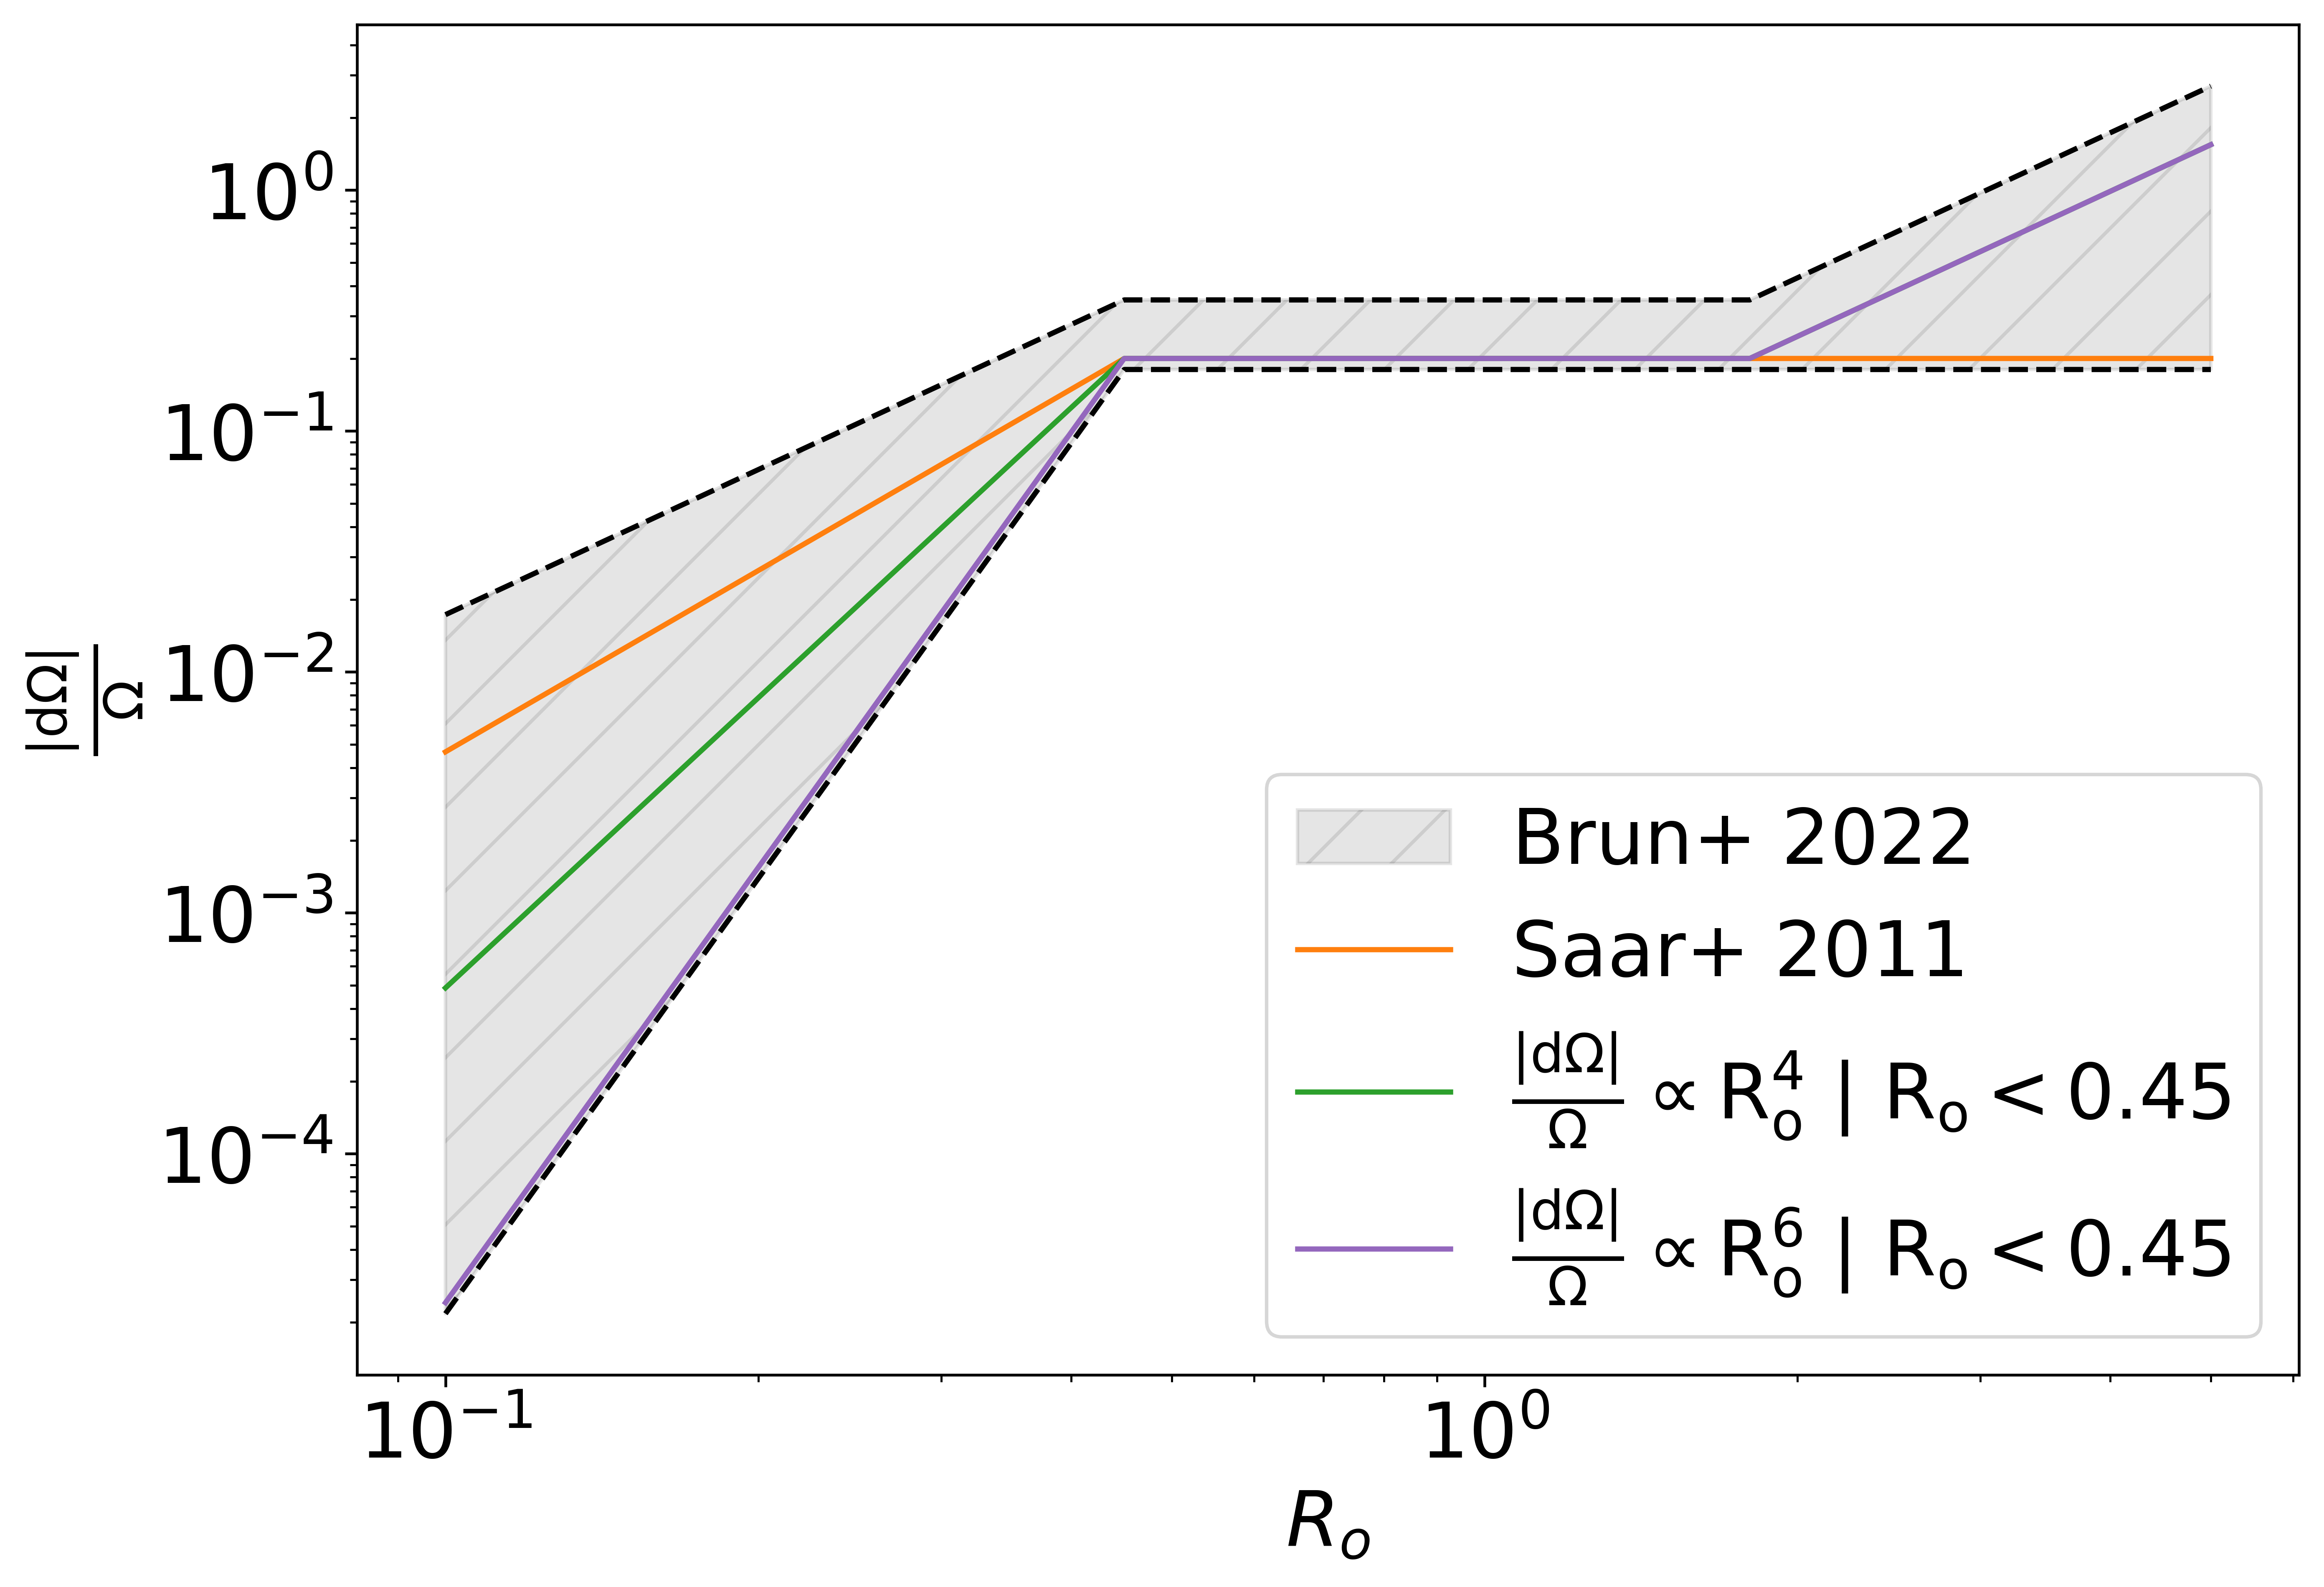
\includegraphics[width=\textwidth]{Figures/rot_gap_figures/comparison_diffrot.png}
 \caption[The relationships between latitudinal differential rotation and the stellar $R_o$ adopted in this work.]{
 	The relationships between latitudinal differential rotation and the $R_o$ adopted in this work. We compare the observationally derived relation from \citet{saar_starspots_2011} (Equation \ref{eq:rot_saar}, orange) and two steeper relations (Equations \ref{eq:rot_pow4} and \ref{eq:rot_pow6}, green and purple, respectively). The scale of differential rotation is greater for the latter two relations. Further, the scale of equator-slow differential rotation grows for $R_o\ \geq \ 2$. All three relations are consistent with the magnetohydrodynamic investigations into stellar differential rotation from \citet{brun_powering_2022}.
}
 \label{fig:compar_diffrot}
\end{figure}

We adopt a second-order equator-fast differential rotation profile with the rotation rate with latitude, $\theta$,
\begin{equation}
 \label{eq:obs_eq}
 \Omega\left(\theta\right) = \Omega_{\rm{eq}} - \frac{\Delta \Omega}{\sin^2 60^{\circ}} \sin^2{\theta}
\end{equation}
where the factor $\frac{1}{\cos^2{60^{\circ}}}$ ensures that the rotation rate is $\Delta \Omega + \Omega_{\rm{eq}}$ at $\theta \ = \ 60^{\circ}$ (from the definition of $\Delta \Omega$).
Given the equatorial rotation rate, this provides us with our expression for our stars' latitudinal differential rotation profile.

Calculating the observed rotation rate, and thus the observed rotation period, from this distribution requires some thought.
We calculate the observed rotation rate from the integral of the rotation rate distribution with $\theta$ divided by the surface area both over the maximum and minimum latitudes that the spots are expressed,
Indeed, this value does not directly map to what would be measured by analysing the light curve. 
This is because, as suggested in \citet{aigrain_hare_2015}, the measured rotation period of stars can be dominated by stochastic, long-lived large stellar spots, so two stars with the same underlying spot probability distribution can have widely different measured periods, depending on when they are observed.
Therefore, our calculation of the observed period here is a qualitative representation of the effect of latitudinal differential rotation on the measured rotation period.

An accurate prescription for variations in the latitudinal distribution of the stellar spots is also unknown.
The latitudinal distribution of stellar spots on the surface of the Sun is well known \citep[see, e.g.,][]{maunder_note_1904,hathaway_solar_2015}.
While we could adopt a solar distribution, this does not account for variations between stars.
For example, the latitudinal distribution of active regions varies along the stellar magnetic cycle \citep[see, e.g.,][ and references therein]{grijs_stellar_2021}.
Further, adopting such a distribution would not account for star-to-star variations with stellar mass, equatorial rotation rate, and the scale of differential rotation both radially and latitudinally.
For this reason, the treatment of the distribution of stellar spots is a major source of uncertainty in our work.
For now, we adopt a uniform distribution of stellar spots between the latitudes of $0^{\circ}$ and $60^{\circ}$.

We will also assume here that all stars in our sample are viewed equator-on.
While this is not the case for all stars, the rotation period gap is not an effect of the observation angle.
Line-of-sight differences due to stellar inclinations can also introduce biases to the measured rotation periods.
Stars must be viewed close to equator-on for stellar spots to introduce significant variations to the light curve as a star rotates.
Further, inclination angles are uniformly distributed in $\cos{i}$, and therefore, most stars with measured rotation periods must be close to equator-on.

The observed rotation rate is then
\begin{equation}
\label{eq:inte}
	\Omega_{\rm{obs}} = \int^{\theta_{\rm{max}}}_{\theta_{\rm{min}}} \Omega(\theta) \cos(\theta)^2 \rm{d}\theta \ / \ \int^{\theta_{\rm{max}}}_{\theta_{\rm{min}}} \cos(\theta)^2 \rm{d}\theta,
\end{equation}
where rotation rate is independent of radius and azimuthal angle, and their contributions cancel.
Here $\theta_{\rm{max}}$ and $\theta_{\rm{min}}$ are the upper and lower bounds of the distribution of spots on the surface of the star.
The factor $\cos(\theta)^2$ arises by accounting for the angle between the surface normal and line-of-sight ($\cos(\theta)$) and the spherical coordinate Jacobian ($\cos(\theta)$).
As the rotation profile is symmetric about the equator of rotation, we only need to calculate the contribution to the rotation rate in one hemisphere.

We begin by comparing the effect of each of the chosen relations between differential rotation and $R_o$ on the observed rotation period of a $0.7 M_{\odot}$ star in Figure \ref{fig:comp_per}.
Latitudinal differential rotation introduces significant biases to the observed rotation periods.
The number of stars with similar observed rotation periods is related to the gradient of $P_{\rm{obs}}$ against $P_{\rm{eq}}$: larger gradients result in an under-density of observations while smaller gradients result in an over-density of observations both relative to the equatorial period distribution.
The growth of differential rotation below $R_o < 0.45$ occurs where $P_{\rm{eq}} < 15$ d.
Steeper relations of $R_o$ with the scale of differential rotation in this domain result in a quicker growth in observed rotation periods for the same equatorial rotation period.
The steeper the growth of the observed rotation period, the lower the number of stars that would be observed with that rotation period.
The transition from equator-fast to equator-slow differential rotation is shown at $P_{\rm{eq}} \ \sim \ 80$ d.

\begin{figure}
\centering
 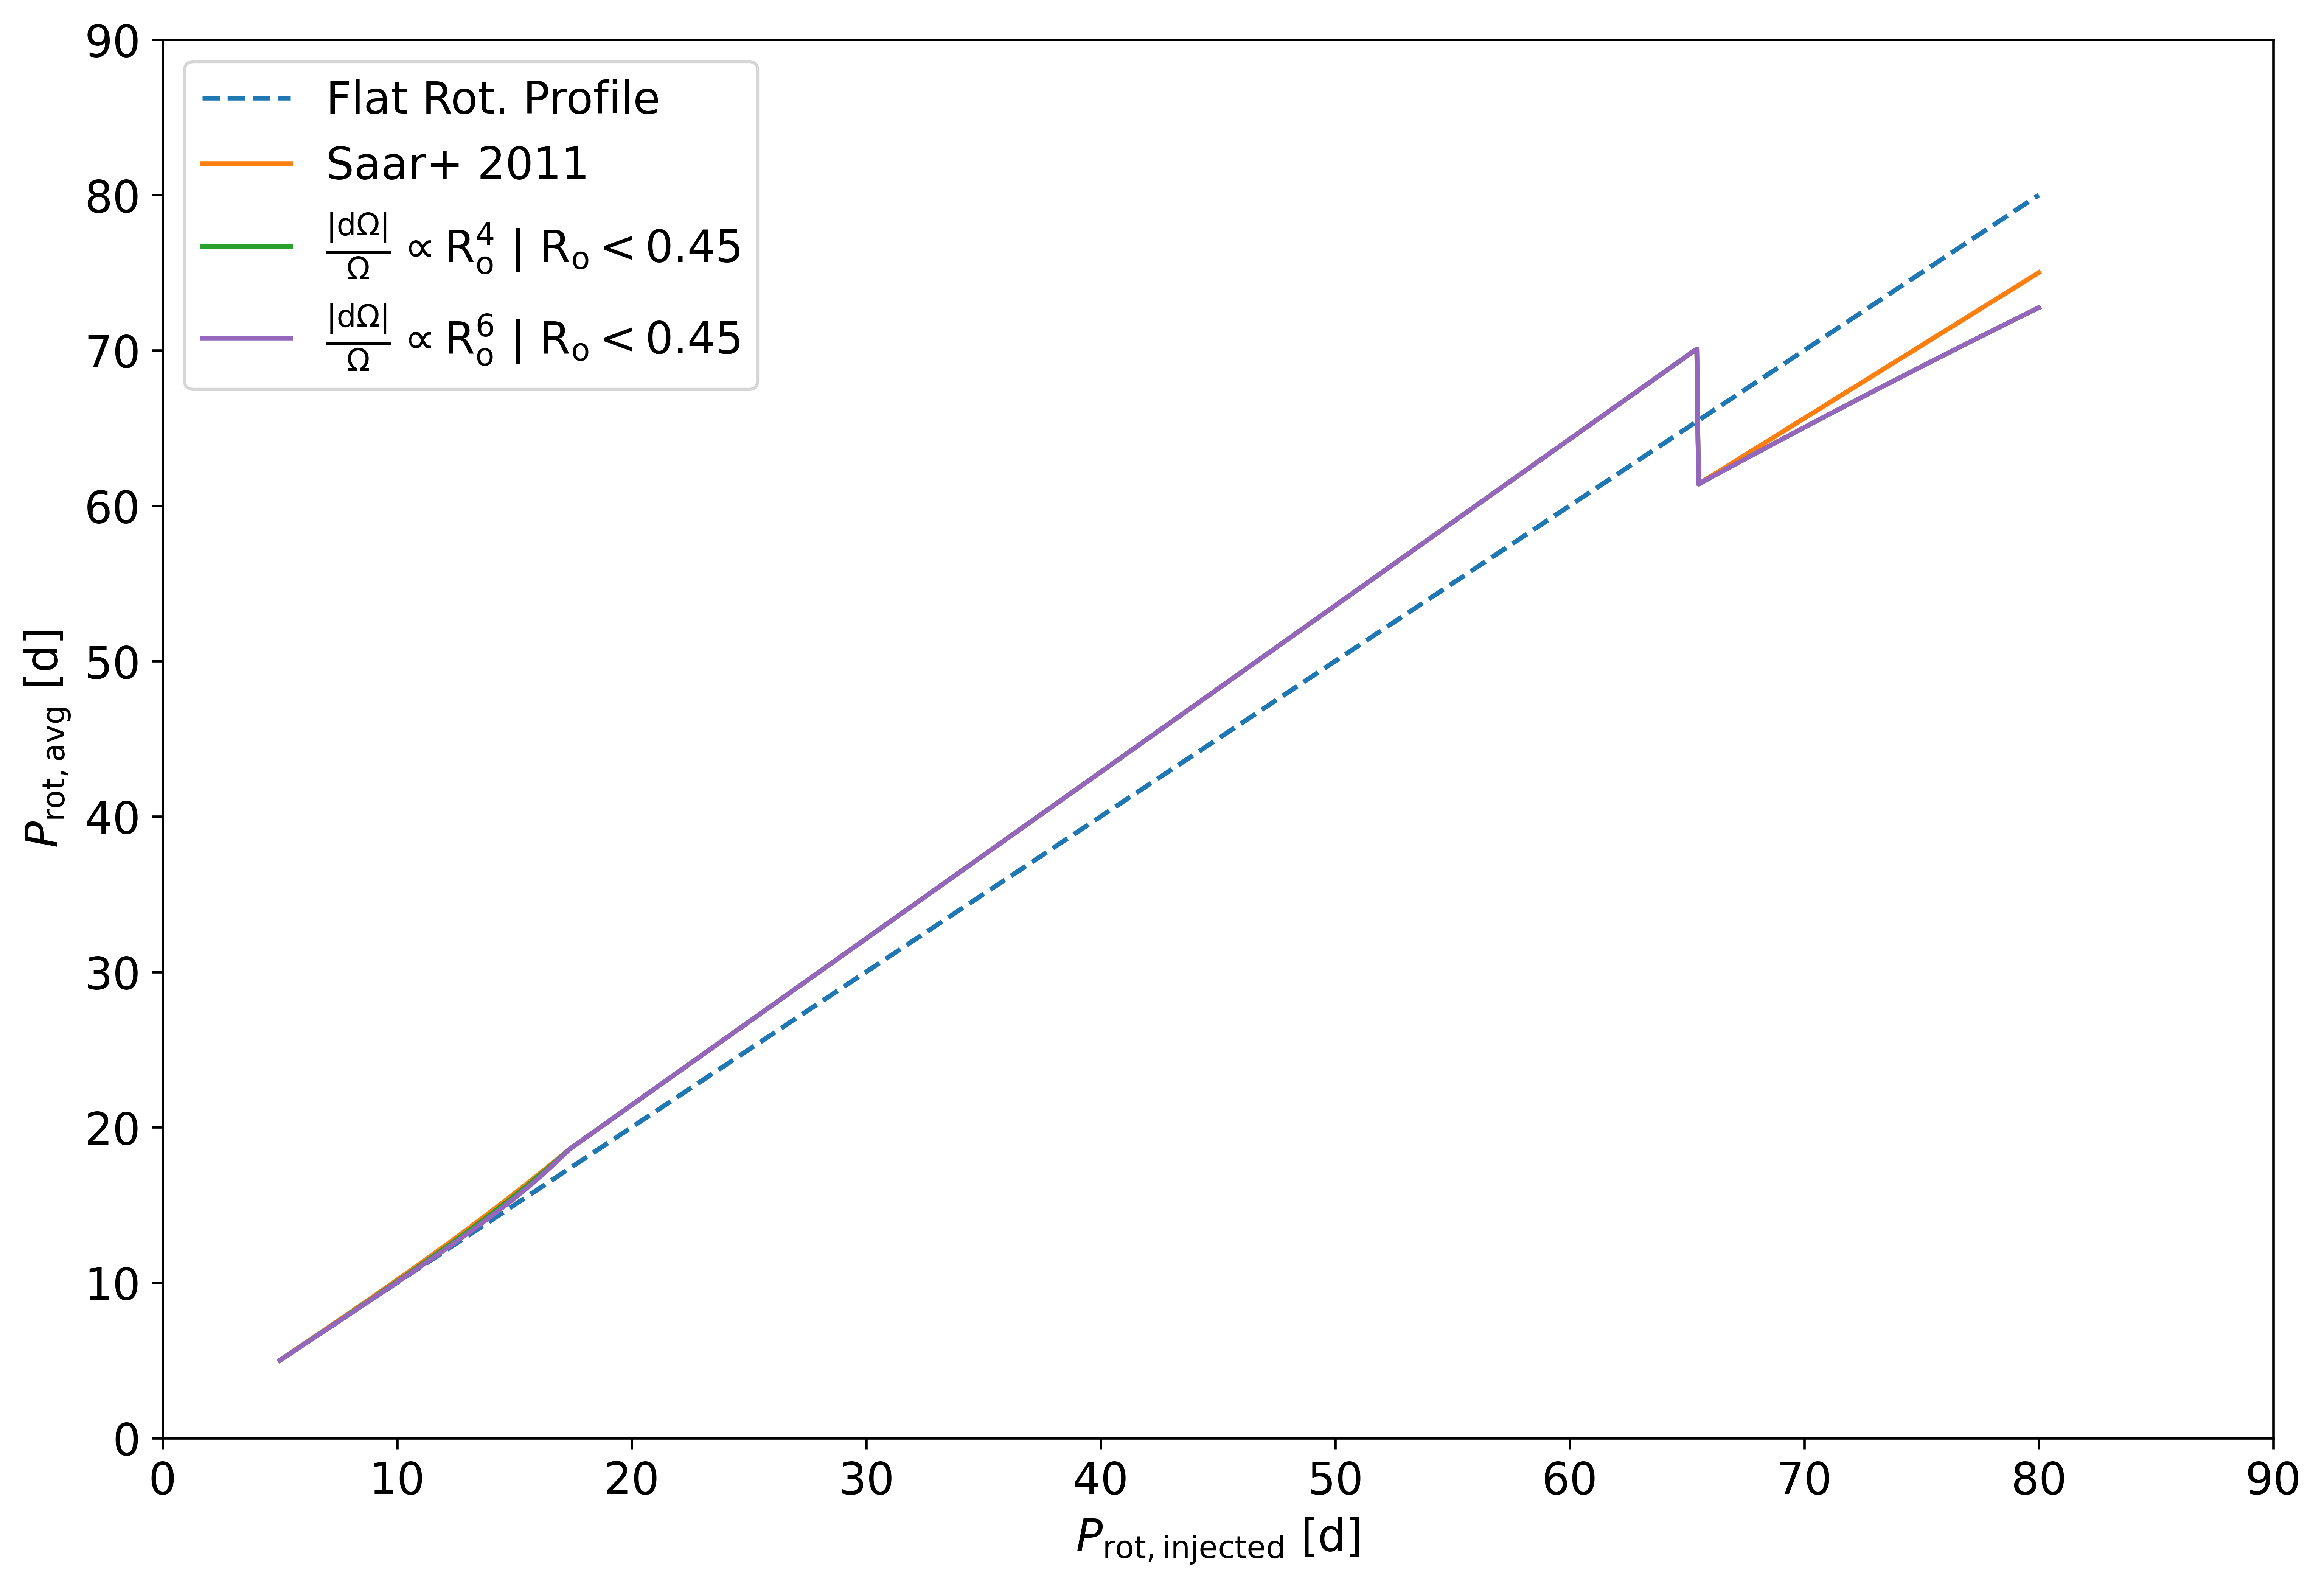
\includegraphics[width=\textwidth]{Figures/rot_gap_figures/comparison_observed_rot_periods.png}
 \caption[The effect of the differential rotation on the observed rotation period of a 0.7 $M_{\odot}$ against equatorial rotation period.]{
 	The effect of the differential rotation on the observed rotation period of a 0.7 $M_{\odot}$ star against the equatorial rotation period. Here, the colour of the relations corresponds to the adopted differential rotation relation in Figure \ref{fig:compar_diffrot} compared to the observed rotation profile of a latitudinally-flat rotating star (blue), where the equatorial rotation period is the observed rotation period. At $R_o<0.45$ for equatorial rotation periods ($P_{\rm{eq}}$) less than 15 days, it is evident that steeper relations between $R_o$ and the scale of differential rotation lead to more rapid growth in observed rotation periods for the same equatorial rotation period. Moreover, a steeper growth in the observed rotation period corresponds to a lower number of observed stars with that particular rotation period. The transition from equator-fast to equator-slow rotation occurs at $P_{\rm{eq}} \ \sim \ 80$ days. The transition from the observed rotation period being greater than the equatorial rotation period results in a larger number of stars observed with similar rotation periods compared to the equator fast-regime \textbf{Inset:} The fractional period difference between the observed and equatorial rotation periods. The relation observed in this Figure is the same as is observed in Figure \ref{fig:compar_diffrot} but highlights the variance in the growth of the difference between the two steep relationships (green and purple), which is not visible when just comparing the observed and equatorial rotation periods. Despite being unable to differentiate between the two in this Figure, we will find that they introduce significant variations to the observed rotation period distribution.}
 \label{fig:comp_per}
\end{figure}

Now, we consider how the bias to rotation periods brought about by differential rotation affects the observed rotation period distribution.
To do this, we assume a sample of stars that are uniformly distributed in effective temperature $\mathcal{U}\left(3500,6000\right)$ and equatorial period $\mathcal{U}\left(0,55\right)$ days, where $\mathcal{U}\left(a,b\right)$ denotes a uniform prior between $a$ and $b$.
The bounds of these distributions are not physically motivated; they only need to include the regimes where $R_o \ = \ 0.45$ and $2$ to observe the effect that the transitions between latitudinally-flat, equator-fast, and equator-slow rotation have on the observed rotation period distribution.
We draw 100,000 effective temperatures and equatorial periods from these distributions and calculate the observed rotation periods under the adopted relationships between differential rotation and $R_o$ (Equations \ref{eq:rot_saar}, \ref{eq:rot_pow4}, and \ref{eq:rot_pow6}).
We plot the equatorial period and observed rotation periods under each of these relations as a 2D histogram in Figure \ref{fig:create_gap}.
We have also indicated in each panel the transitions between latitudinally-flat to significant equator-fast differential rotation (dashed line, $R_o = 0.45$), and equator-fast to equator-slow differential rotation (dashed line, $R_o = 2$).
Our models predict a dearth of observations, coincident with the intermediate period gap due to the transition from latitudinally-flat to significant equator-fast differential rotation.
This can be seen by comparing the top left panel to the other three.
The distinctness, or rather the decrease in density of stars within the gap, increases with the power on $R_o$ (2, 4, and 8 for Equations \ref{eq:rot_saar}, \ref{eq:rot_pow4}, \ref{eq:rot_pow6} respectively) within the transition between latitudinally-flat to significant equator-fast differential rotation, $R_o \leq 0.45$.
We also find that our models predict an over-density of observations where the transition from equator-fast to equator-slow latitudinal differential rotation occurs ($P \ = \ 25$ d, $T_{\rm{eff}} \ = \ 6000 \ K$).

\begin{figure}
\centering
 \includegraphics[width=\textwidth]{Figures/rot_gap_figures/create_gap.png}
 \caption[The effect of differential rotation on the observed rotation period distribution.]{The effect of differential rotation on the observed rotation period distribution of a sample of stars with uniformly distributed effective temperature and equatorial rotation period. We show the 2D histograms of the equatorial rotation period (top left) against effective temperature as well as the observed rotation periods under each of the adopted differential rotation relations: Equations \ref{eq:rot_saar} (top right), \ref{eq:rot_pow4} (bottom left), and\ref{eq:rot_pow6} (bottom right). The transitions between latitudinally-flat to significant equator-fast differential rotation ($R_o = 0.45$), and equator-fast to equator-slow differential rotation ($R_o = 2$) are shown in dashed and dotted lines, respectively. Our models predict a dearth of observations, coincident with the intermediate period gap due to the transition from latitudinally-flat to significant equator-fast differential rotation and an over-density of observations at the transition from equator-fast to equator-slow rotation.}
 \label{fig:create_gap}
\end{figure}

\subsection{A physically motivated synthetic sample of observed rotation periods}

We require a physically motivated synthetic sample of rotation periods to compare our model observed rotation periods to the measured rotation period distribution of \citet{mcquillan_rotation_2014}.

We adopt equatorial rotation periods ($P_{\rm{eq}}$) from cluster-tuned rotational isochrones for a given stellar age and mass (these rotational isochrones are shown in Table A1 in \citet{spada_competing_2020}).
The ages of these isochrones are limited to the solar age (4.5 Gyr), placing an upper limit on the age of our population.

The use of their rotation periods in this work warrants some discussion.
In their work, they propose a model of rotation period evolution that a wind braking and 2-zone (core and surface) mass-dependent angular momentum transport.
They tune the wind-braking and core-envelope coupling timescale through the measured rotation periods of young clusters: Pleiades (120 Myr, \citep{rebull_rotation_2016}), Praesepe (700 Myr, \citep{douglas_poking_2017, douglas_k2_2019}), and NGC 6811 (1 Gyr, \citep{curtis_temporary_2019}) as well as the rotation period of the Sun (4.5 Gyr).
The adopted rotation period of the Sun in their work is also the scaled average rotation period of the latitudinally differentially rotating surface scaled by the latitudinal distribution of stellar spots rather than the equatorial rotation period (26.9 d).
This value is notably much closer to the Sun's equatorial rotation period ($\sim 25$ d) than the polar rotation period ($\sim 31$ d).

If, indeed, we are correct that latitudinal differential rotation introduces biases to the measured rotation period, then tuning models using measured rotation periods and not accounting for the bias (that latitudinal differential rotation may introduce) could result in inaccurate prescriptions of the evolution of rotation.
The measured rotation periods used to tune our generative model of what we assume are equatorial rotation periods are shown in Figure \ref{fig:com_gap_clus}.
We have also plotted the line $R_o \ = \ 0.45$, where we assume equator-fast latitudinal differential rotation becomes significant and impacts the observed rotation period.
Most high-temperature ($>$ 5000 K) Pleiades and Praesepe members lay above this line.
The measured rotation periods of high-mass stars in their work are not equatorial but, in fact, already the biased, measured rotation periods.
We will introduce a bias to our sample's potentially already biased rotation periods for high-mass stars.
On the other hand, low-mass stars ($>$ 5000 K) lay below this line.
The measured rotation period of these low-mass stars is the equatorial rotation period, and the model may be tuned to only the equatorial rotation periods of low-mass stars.
Older ($>$ 1 Gyr) low-mass rotation periods output by their model are projections of equatorial rotation periods.
Given that the introduced dearth is most apparent for low-mass stars older than 1 Gyr, we believe adopting these values as the equatorial rotation periods is appropriate.

We also compare in this Figure the rotation period distributions of each cluster against the rotation periods of the \citet{spada_competing_2020} model evaluated at the representative ages of each of the clusters (dashed lines).
While this model generally agrees with the high-mass members of the clusters, it was tuned to (Pleiades, Praesepe, NGC 6811), as well as the high-mass members of NGC 6819, it significantly over-predicts the rotation periods of low-mass stars.
This is especially pervasive for stars with effective temperatures less than 4000 K.
This results in very few low-mass stars with rotation periods that place them on the lower branch of the intermediate period gap and an over-density of measured rotation periods of low-mass stars.
We, therefore, exclude stars with effective temperatures less than 4000 K from our synthetic sample. 
While this leaves us with a small range of effective temperatures that we adopt in our work, where the output rotation periods from their model are the equatorial rotation periods, the gap is still apparent in this range: we can see, qualitatively, if the bias introduced by differential rotation produces a gap consistent with the measured rotation periods.
We will revisit this assumption in reference to our conclusions in Section \ref{sec:discussion}.

\begin{figure}
\centering
 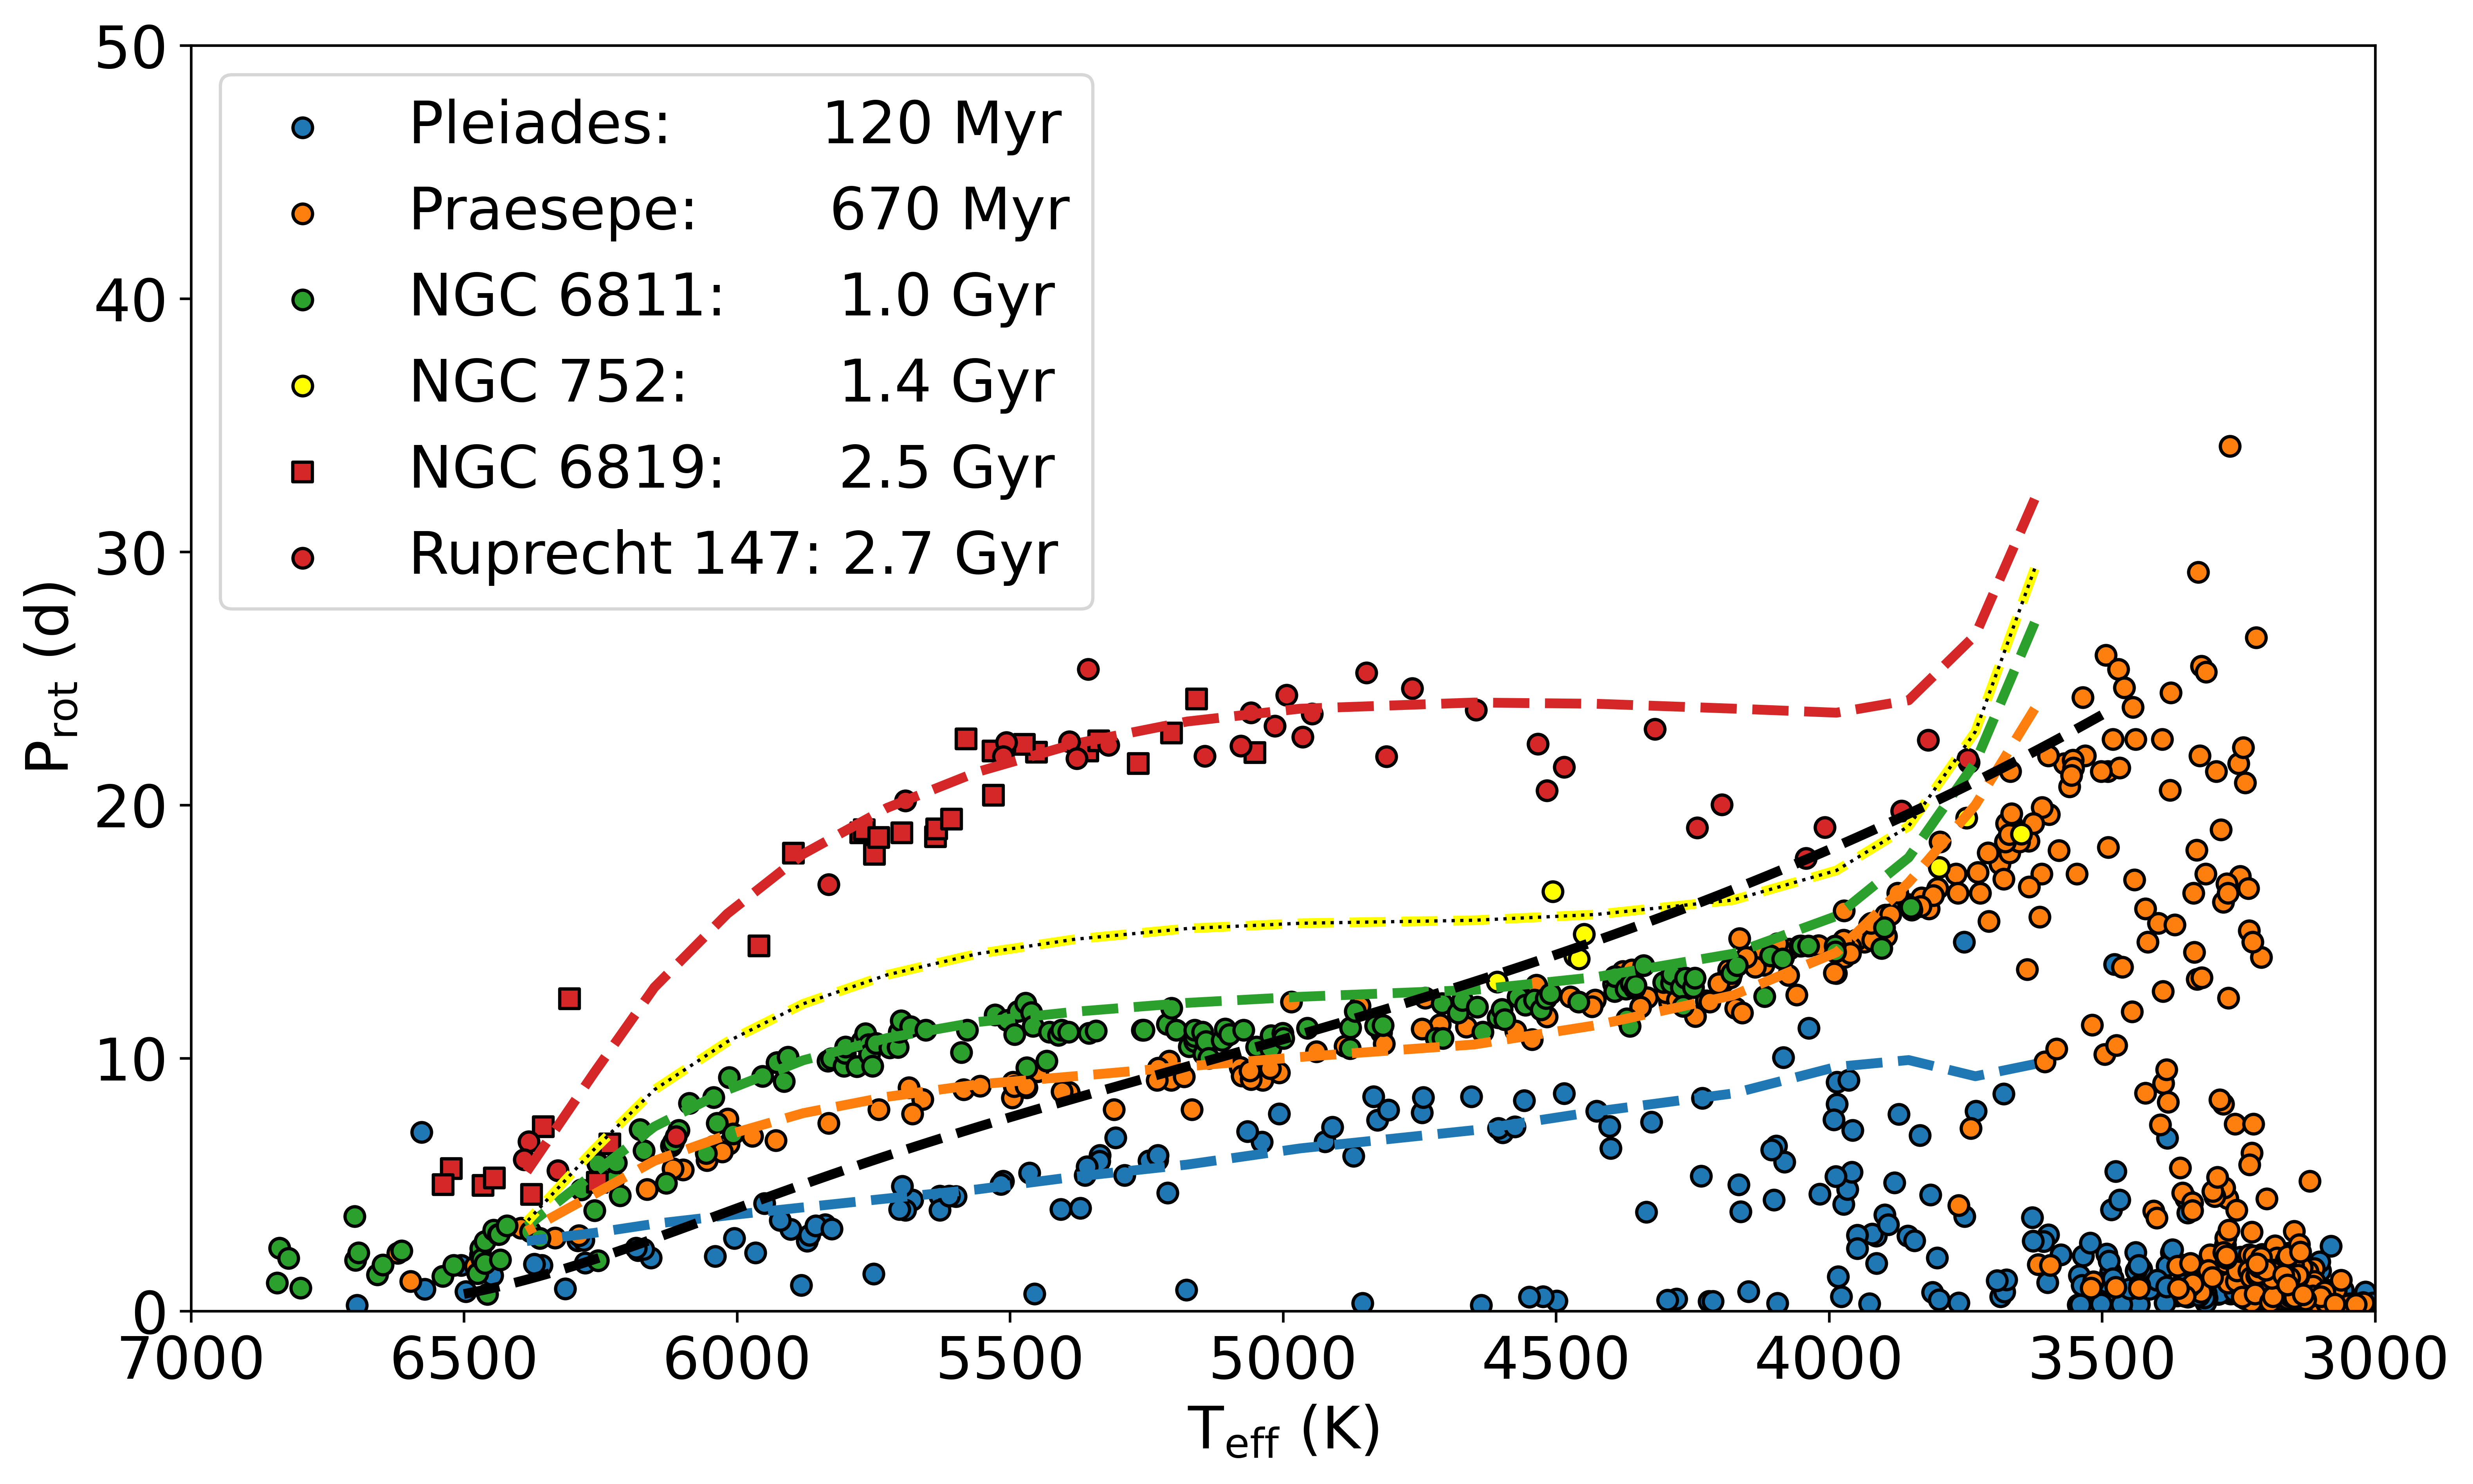
\includegraphics[width=\textwidth]{Figures/rot_gap_figures/com_gap_clus.png}
 \caption[Cluster rotation periods distributions against effective temperature.]{Scatter plot of clusters, Pleiades (120 Myr, blue \citep{rebull_rotation_2016}), Praesepe (orange, 700 Myr, \citep{douglas_poking_2017, douglas_k2_2019}) and NGC 6811 (green, 1 Gyr, \citep{curtis_temporary_2019}), used to tune the rotational isochrones adopted in this work \citep{spada_competing_2020} as well as the rotational period distributions of NGC 752 (yellow, 1.4 Gyr), NGC 6819 (red squares, 2.5 Gyr - projected forward to 2.7 Gyr: scaled through Skumanich spin-down, for direct comparison with the Ruprecht 147 sample, \citep{meibom_kepler_2011}), and Ruprecht 147 (red circles, 2.7 Gyr, \citep{curtis_when_2020}) against effective temperature. \textbf{Dashed lines:} \citep{spada_competing_2020} rotational isochrones evaluated at the ages of each stellar cluster and coloured to match the scatter points. We have also shown the line $R_o \ = \ 0.45$ (black dashed), highlighting that the high temperature ($\>$5000K) Pleiades and Praesepe members may have significant latitudinal differential rotation, biasing the measured rotation periods, while low-temperature stars may not. Suggesting that the measured rotation period of these stars is the equatorial rotation period, and adopting the \citet{spada_competing_2020} values as the equatorial rotation periods is appropriate for low-mass stars. We also show the rotation periods evaluated by the \citet{spada_competing_2020} model evaluated at the representative ages of each cluster (dashed lines coloured by the cluster of the same age).
While this model generally agrees with the high-mass members of the clusters, it was tuned to (Pleiades, Praesepe, NGC 6811), as well as the high-mass members of NGC 6819, it significantly over-predicts the rotation periods of low-mass stars.
This is especially pervasive for stars with effective temperatures less than 4000K.}
 \label{fig:com_gap_clus}
\end{figure}

%add references to the cluster rotation periods and discuss the discrepancy between the observed NGC6811 and Ruprecht 147 rotation periods. 


We generate 30,000 main-sequence and early post-main-sequence stars with various mass, age, metallicity and equatorial rotation period values.
We drew masses from a uniform mass function $\mathcal{U}\left(0.65,1\right)$ $M_{\odot}$.
This limits our range of masses to those with a convective surface and radiative core and an effective temperature greater than 4000 K.
The gap is apparent in this range ($T_{\rm{eff}} \ < \ 5000$ K).
The choice of a uniform initial mass function here is motivated by the selection function of the \kepler\ mission being biased towards the observation of brighter stars.
We assume that the selection function effectively cancels out the bias towards a larger number of low-mass stars of physically motivated initial mass functions like a Salpeter initial mass function.

%todo:check this with Andy
Metallicity is drawn from a distribution to approximately reflect what is observed in the Milky Way. Specifically, we defined a variable $\phi$ to be drawn from a Beta distribution
\begin{equation}
 \phi \sim \mathcal{B}\left(\alpha=10, \beta=2\right)
\end{equation}
and applied a transform from $\phi$ to [Fe/H] by requiring the metallicities be bounded between $[\mathrm{Fe/H}]_\mathrm{min} =-2$ and $[\mathrm{Fe/H}]_\mathrm{max} = +0.5$. We also required that the mode of $\phi$, defined as $\frac{\alpha - 1}{\alpha + \beta - 2}$ for a Beta distribution, occurs at Solar metallicity. This leads to the transform:
\begin{equation}
 [\mathrm{Fe/H}] = \left(\frac{}{}[\mathrm{Fe/H}]_\mathrm{max}-[\mathrm{Fe/H}]_\mathrm{min}\right)\left(\phi - \frac{\alpha - 1}{\alpha + \beta - 2}\right) \quad .
\end{equation}

The stars we generate mock data for in this work span from the ZAMS to low-luminosity subgiants.
We draw equivalent evolutionary phase (EEP) values\footnote{The principle of the EEPs is to define physically significant stages in stellar evolution (e.g. core-H burning, core-H depletion, RGB), and then subdivide each of these stages into a number of equal steps. See \citet{morton_isochrones_2015} for a more in-depth discussion of the definition of these values.} from a uniform distribution of EEPs $U\sim(200,450)$.
The bounds of this range (200 and 450) represent the ZAMS and the low-luminosity subgiant phase, respectively.
Using the EEP, mass, and metallicity, we interpolate a position along the MIST stellar isochrones \citep{morton_isochrones_2015} to calculate the expected \teff \ , and luminosity of each star as well as the post-ZAMS age.
This results in a population biased towards younger ($<$ 1 Gyr) stars.
We found that after calculating the equatorial rotation periods under this population, the rotational period distribution had a much higher density of observations of low rotational periods than the \citet{mcquillan_rotation_2014} sample, ensuring comparison between the two is not biased by the choice of age distribution.
We sampled our population until we had a population uniform in age between 300 Myr and 4.5 Gyr, ensuring the sample was on the slow-rotator sequence but younger than the solar age.
From these parameters, we can then calculate the observed rotation periods of our synthetic sample.

\section{Results}
\label{sec:results}

The resulting distributions of observed rotation periods (blue, orange, green and purple) relative to the measured rotation period distribution of \kepler{} \citep{mcquillan_rotation_2014} (black) are shown in Figure \ref{fig:comp_dist}.
Here, the colour of each distribution corresponds to the same colour, showing the relation between differential rotation and $R_o$ in Figure \ref{fig:compar_diffrot} and blue corresponds to the equatorial, or latitudinally-flat rotation profile, observed rotation period.

Figure \ref{fig:comp_hess} shows how the adopted relations impact the rotation period distributions.
The left column shows the 2D histogram of the \citet{mcquillan_rotation_2014} measured rotation period distribution.
In the middle column, we show the 2D histogram of the observed rotation period distributions under the adopted relations between latitudinal differential rotation and $R_o$.
From top to bottom panel, we show the equatorial rotation periods from our generative model (with no latitudinal differential rotation), then under the \citet{saar_starspots_2011} Equation (\ref{eq:rot_saar}) differential rotation relation, then with the Equation (\ref{eq:rot_pow4}) model, and finally with the Equation (\ref{eq:rot_pow6}) model.
These panels correspond to the blue, orange, green, and purple distributions in Figure \ref{fig:compar_diffrot} respectively.
All of the panels in the left two columns are coloured by the number of stars in each bin for each panel: N$_{\rm{Obs.}}$, the number in each bin of the \citet{mcquillan_rotation_2014} sample, for the left column and N$_{\rm{Mod.}}$, the number in each bin of the various models, for the middle column.
In the right column, we show the difference between the distributions through N$_{\rm{Obs.}}$ and N$_{\rm{Mod.}}$ for each adopted relation.
Darker colours correspond to regions where the model over-predicts observations and lighter where the model under-predicts observations.

Like in Figure \ref{fig:create_gap}, our models predict a dearth of observations, coincident with the intermediate period gap as a result of the transition from latitudinally-flat to equator-fast differential rotation at $R_o = 0.45$.
We observe that the model that adopts latitudinal differential rotation when calculating the observed rotation period reduces the disparity between the model observed and measured rotation period distributions: compare the top panel to the bottom three in the right column of Figure \ref{fig:comp_hess}.
Further, the increased density of observations of stars just above the intermediate period gap in the \kepler{} sample is reproduced under this model, unlike a model of extreme magnetic braking to explain the gap.
We again observe that increases with the power on $R_o$ (2, 4, and 8 for Equations \ref{eq:rot_saar}, \ref{eq:rot_pow4}, \ref{eq:rot_pow6} respectively) increase the distinctiveness (relative decrease in density of observations) of the gap.
We also find that all models predict an over-density of stars where the transition from equator-fast to equator-slow latitudinal differential rotation occurs ($\log P_{\rm{rot}}/d = 1.2$, $T_{\rm{eff}} = 6000 \ K$), coinciding with the long-period pileup.
The model also predicts this over-density with no differential rotation, but the shape of the distributions in this domain do not agree.
When we introduce differential rotation, however, the shape of the upper edge of the model observed rotation period distributions closely matches the shape of the measured rotation period distribution.
The coincidence of the position of the over-density predicted by our model and the long-period pileup may suggest that, in fact, the cause of the long-period pileup is this transition.


\begin{figure}
\centering
 \includegraphics[width=\textwidth]{Figures/rot_gap_figures/comp_dist.png}
 \caption[The observed rotation period distributions of the synthetic sample of stars given various relations between latitudinal differential rotation and $R_o$ overlayed over the distribution of measured rotation periods of the \kepler{} sample from \citet{mcquillan_rotation_2014}.]{
 	The observed rotation period distributions of the synthetic sample of stars given various relations between latitudinal differential rotation and $R_o$ overlayed over the measured distribution of rotation periods of the \kepler{} sample from \citet{mcquillan_rotation_2014} (black). Here, the coloured observed rotation period distributions correspond to the various differential rotation relations adopted in this work, as seen in Figure \ref{fig:compar_diffrot}. The latitudinally-flat (blue, top left) sample reflects the equatorial rotation periods of our sample considered in this work. We observe no intermediate period gap in this synthetic sample of stars without differential rotation. 
We observe the effects of latitudinal differential rotation on the observed rotation period. We tentatively observe a dearth of observations at the transition between latitudinally-flat ($R_o \ < \ 0.45$) and equator-fast rotation, which occurs precisely at the location of the intermediate period gap.
To more thoroughly investigate the introduced variations, we have plotted the 2D histograms of these distributions to qualify and make comparisons between the measured and model observed rotation distributions in Figure \ref{fig:comp_hess}.}
 \label{fig:comp_dist}
\end{figure}

\begin{figure}
\centering
 \includegraphics[width=\textwidth]{Figures/rot_gap_figures/comp_hess_up.png}
 \caption[2D histograms of measured and the synthetic observed rotation period distribution assuming various relations between the scale of differential rotation and $R_o$ and the difference between the two.]{
2D histograms of measured and the synthetic observed rotation period distribution assume various relations between the scale of differential rotation and $R_o$ and the difference between the two.
\textbf{Left:} 2D histogram of the \citet{mcquillan_rotation_2014} rotation period distribution.
\textbf{Middle:} 2D histogram of the measured rotation period distributions under the adopted relations between latitudinal differential rotation and $R_o$. From the top to the bottom panel, we show the equatorial rotation periods from our generative model (with no latitudinal differential rotation), then the relation under the \citet{saar_starspots_2011} differential rotation relation (Equation \ref{eq:rot_saar}), then with two steeper but physically probable (Equation \ref{eq:rot_saar}) and two model-motivated \citep{brun_powering_2022} scale of differential rotation relations Equations \ref{eq:rot_pow4}, \ref{eq:rot_pow6}.
These distributions correspond to the blue, orange, green, and purple distributions in Figure \ref{fig:compar_diffrot} respectively.
All of the panels in the two left columns are colour by the number of stars in each bin: N$_{\rm{Obs.}}$, the number in each bin of the \citet{mcquillan_rotation_2014} sample, for the left column and N$_{\rm{Mod.}}$ for the middle, the number in each bin of the various models. \textbf{Right:} The difference between the distributions: N$_{\rm{Obs.}}$ - N$_{\rm{Mod.}}$ for each adopted relation.
Darker colours correspond to regions where the model over-predicts observations and lighter where the model under-predicts observations. Accounting for differential rotation when determining the expected observed rotation periods of stars introduces a decrease in the density of observations where significant equator-fast differential rotation arises.
The dearth is coincident with the intermediate period gap. We find that the larger the power in the relation between $\frac{\Delta\Omega}{\Omega_{\rm{eq}}}$ and $R_o$ below the transition to a saturated scale of differential rotation (2, 4, and 8 for Equations \ref{eq:rot_saar}, \ref{eq:rot_pow4}, \ref{eq:rot_pow6} respectively), the more apparent the dearth becomes. Our models predict an over-density of stars where the transition from equator-fast to equator-slow latitudinal differential rotation occurs ($\log P_{\rm{rot}}/d \ = \ 1.2$, $T_{\rm{eff}} \ = \ 6000$ K) which aligns with the position of the long-period pileup.}
 \label{fig:comp_hess}
\end{figure}

\section{Discussion}
\label{sec:discussion}

In this Chapter, we have proposed a novel explanation for the intermediate period gap: the growth equator-fast differential rotation near the location of the intermediate period gap and the effect that this has on the observed rotation periods of stars.
We propose this explanation for the intermediate period gap due to our perceived lack of evidence for other current explanations for the intermediate period gap.
Those two leading theories are that stars in the intermediate period gap drop below the detectability threshold suggested by the drop in photometric variability of stars near the gap or that stars "jump" the intermediate period gap through sudden enhanced magnetic braking.
In Appendix \ref{apndx:magnetic} of this thesis, we have discussed an investigation into evidence against these explanations, which we believe suggests that these explanations are not the underlying mechanism of the intermediate period gap.

In this work, we consider the effect of latitudinal differential rotation on the observed rotation periods of main-sequence stars.
To do this, we developed a model to predict the observed rotation period of stars given models of surface latitudinal differential rotation growth from observational and 2D magnetohydrodynamical simulations of rotating main-sequence stars.
The observations of latitudinal differential rotation and magnetohydrodynamical models of latitudinal differential rotation with $R_o$ agree - suggesting that latitudinal differential rotation grows from latitudinally-flat to equator-fast differentially rotating at a $R_o \approx 0.45$.
Introducing this differential rotation to our calculation of the observed surface rotation period of stars produces a lower density of observations where the differential rotation grows.
We believe that this suggests that the underlying mechanism of the intermediate period gap is the onset of latitudinal differential rotation.
We have investigated several relationships between the scale of growth of latitudinal differential rotation and $R_o$. The qualitatively best-fit relations have a swift growth of $\frac{\Delta\Omega}{\Omega_{\rm{eq}}}$ close to the intermediate period gap (Equations \ref{eq:rot_pow4} and \ref{eq:rot_pow6}).
We found in this work that the distinctness, or rather the decrease in density of stars within the gap, increases with the power on $R_o$ when $R_o \leq 0.45$.

While our model predicts a dearth of observations coincident with the gap, we are hesitant to suggest a prescription for the growth of the scale of differential rotation based on our results.
There is significant degeneracy between several parameters in our work, and there are still many unknowns that we have yet to account for that require future work.

We adopt a constant distribution of stellar spots between a latitude of $0^{\circ}$ and $60^{\circ}$.
The evolution of the latitudinal distribution of stellar spots is unknown, so we will not speculate as to whether changes to this parameter would result in our models reflecting the observed rotational distribution.
However, we will note the effects that variations to this parameter have.
If spots are more concentrated to the equator ($\theta_{\rm{min}} = 0^{\circ}$ and $\theta_{\rm{max}} < 60^{\circ}$) then the observed rotation periods more closely reflect the equatorial rotation periods.
Conversely, if spots are more concentrated toward the poles ($\theta_{\rm{min}} > 0^{\circ}$ and $\theta_{\rm{max}} > 60^{\circ}$), then differential rotation will have a larger impact on the observed rotation period distribution.
The observed rotation periods will be much larger than the equatorial rotation periods.
The variations that those variations make are similar to an increase in the saturated scaling of differential rotation $\left(\frac{\Delta\Omega}{\Omega_{\rm{eq}}}\right)$.
The larger this value, the greater the scale of the dearth region in terms of rotation period.

A more rigorous model of the latitudinal expression of stellar spots and their effect on the measured rotation period of stars is required to determine the effect of latitudinal shear on the measured rotation periods.
Such an analysis could first be completed with non-uniform distributions of stellar spots on the surface of stars from magnetohydrodynamic simulations of rotating stars using a similar analysis to that performed in this work. 
The relation between this work's purported observed rotation periods and measured rotation periods from light curves, including differential rotation, is unclear.
The effect of latitudinal shear on the measured rotation period may, in fact be minimal compared to the effect observed here.

We have adopted a uniform function to draw our stellar masses.
A uniform mass distribution better reflects the mass distribution of the \citet{mcquillan_rotation_2014} sample (a Salpeter initial mass function, for example, predicts an order of magnitude greater number of low-mass stars), but under-predicts the number of high-mass stars relative to low-mass stars.
The probability density distributions generally agree when comparing the effective temperature and luminosity distributions, as seen in Figure \ref{fig:compar_teff_logl}.
We believe that this assumption is sound.
The relative distribution of rotational periods and effective temperatures between the two distributions (measured and model observed), as we have performed in Section \ref{sec:results}, will not be significantly biased by the underlying mass distribution.

\begin{figure}
\centering
 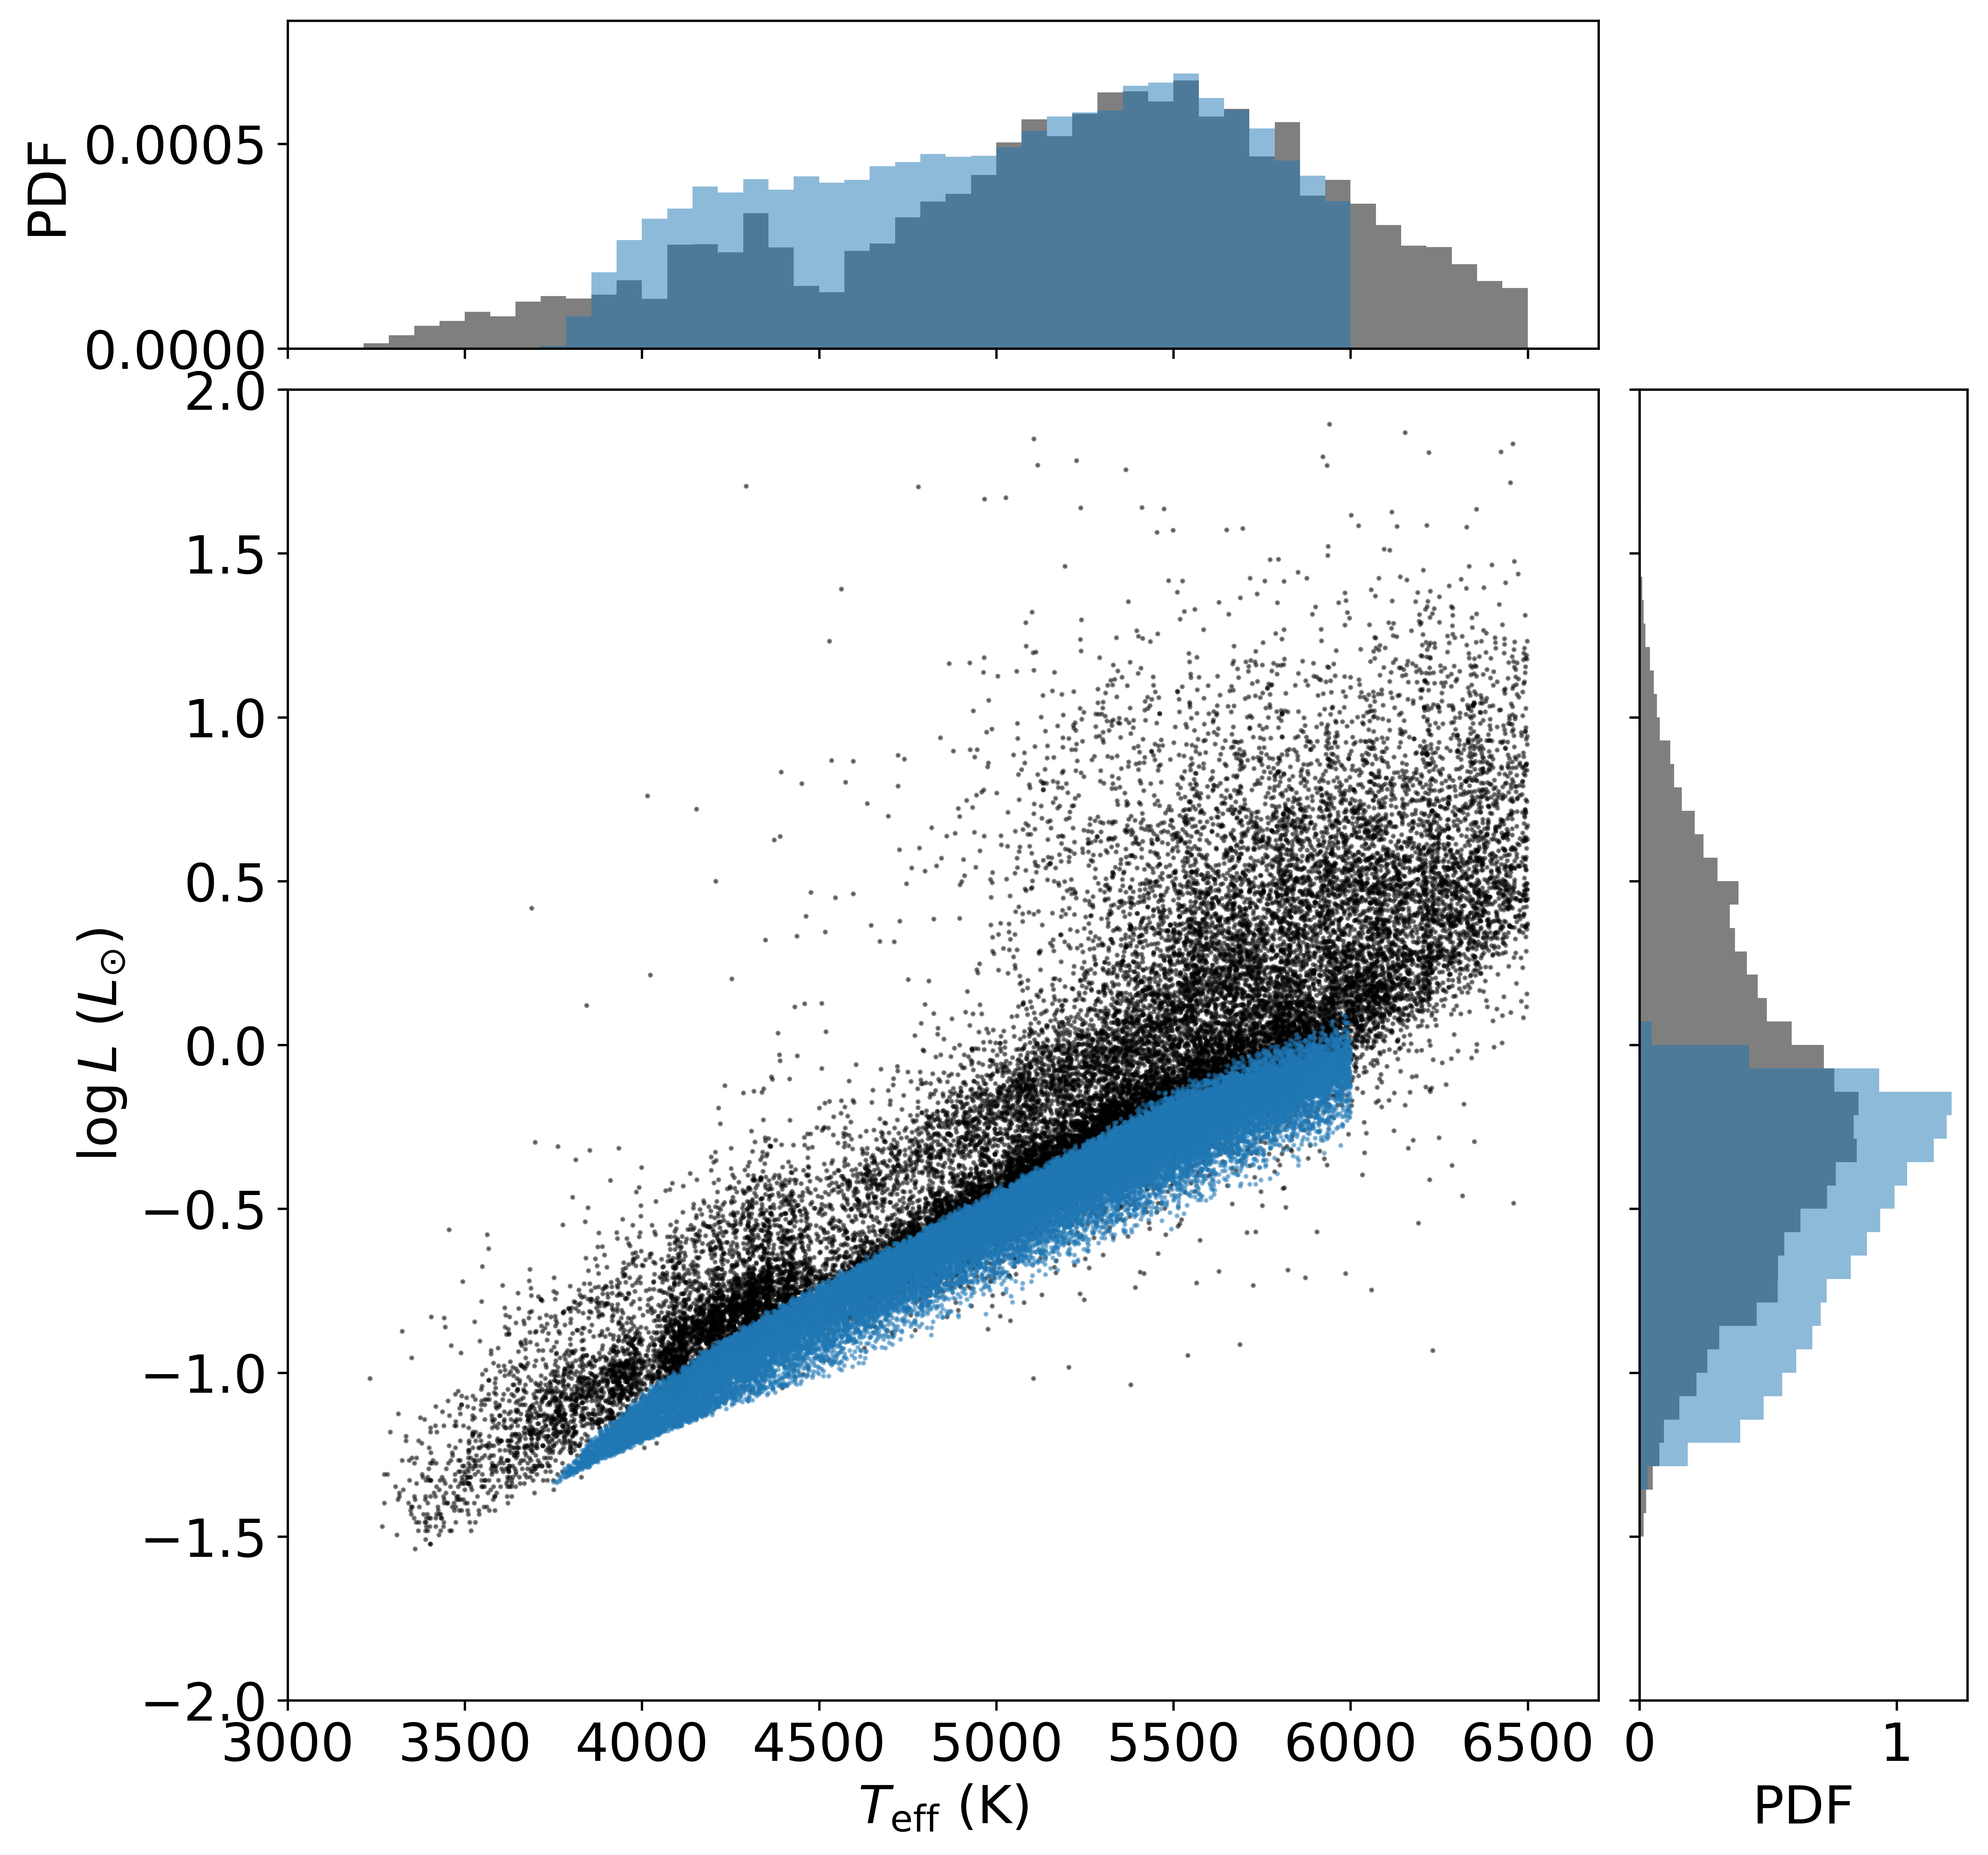
\includegraphics[width=\textwidth]{Figures/rot_gap_figures/compar_dist.png}
 \caption[A comparison between the effective temperature and luminosity distributions of the \citet{mcquillan_rotation_2014} and synthetic sample adopted in this work. ]{A scatter plot of effective temperature and luminosity distributions of the \citet{mcquillan_rotation_2014} (black) and synthetic sample (blue) adopted in this work. On the left and above, we also show the probability density distributions of the luminosity and effective temperature, respectively. The distributions generally agree, suggesting that a direct comparison between the distributions is sound.}
 \label{fig:compar_teff_logl}
\end{figure}

We argued in Section \ref{sec:intro} that a physical model of the intermediate period gap must account for all of the observed features of the gap.
We believe that our model reproduces a number of these features.
The gap definitionally aligns with a line of constant $R_o$, the swift growth of equator-fast latitudinal shear occurs at $R_o$ = 0.45.
The model naturally reproduces the roughly equal density distribution of stars above and below the gap (See the middle columns of Figure \ref{fig:comp_hess}).
Stars above and below the gap are of similar age (assuming Skumanich-like spin-down of the equator rotation rate) but swiftly grow in the observed rotation period.
 As a result, stars above and below the gap would not be significantly observationally distinct and would be of a similar kinematic age.
More theoretical work is required to determine whether some of those features arise due to latitudinal bias.

For example, it is unknown how our model interacts with fully convective stars: the variance of latitudinal shear with $R_o$ of fully convective is unknown.
On the other hand, a feature of the intermediate period gap not currently explained by our results is the decreased \rper{} of stars within the gap relative to the surrounding rotation periods.
We propose a mechanism to explain this feature.
The fractional spot coverage of young, fast rotators ($R_o \ < \ 0.2$) is saturated.
Above this regime, the fractional spot coverage drops rapidly (See Figure 7. in \citet{cao_starspots_2022}).
Latitudinal shear is, however, anticipated to serve as a catalyst for large-scale strong magnetic fields.
Further, latitudinal shear leads to differential twisting of the poloidal field lines, resulting in a bunching of field lines that result in active regions on the surfaces of stars \citep[see, e.g.,][]{berdyugina_starspots_2005, miesch_large-scale_2005, magnetism_brun_2017}
As latitudinal shear grows, we, therefore, speculate that the fractional spot coverage of stars could, in turn, increase, leading to the observed increase in \rper{} above the gap.
We intend to investigate this testable hypothesis by measuring the fractional spot coverage of stars above the gap.
Further work to confirm the mechanism is required with more rigorous methods and theoretical investigations.

Confirmation of this model as the cause of the intermediate period gap using observational data is difficult.
Constraining the scale of latitudinal differential rotation of main-sequence stars appears improbable using current photometric methods \citep[See Section 4.3 of][]{aigrain_hare_2015}.
However potential observations of the differential rotation of nearby stars with Doppler imaging above and below the rotation period gap could be performed.
Observations of significant variance between the latitudinal differential rotation of stars above and below the gap suggest that our model is accurate.
To make a recommendation, a first step in this investigation could be observing the stars seemingly crossing the gap in the nearby open cluster Ruprecht 147 \citep{curtis_when_2020}.

The transition from equator-fast to equator-slow differential rotation is not well characterised in theory or observations.
If this transition does occur, we expect the observed rotation periods of stars to decrease suddenly, resulting in an increased density of observations near this transition.
This work shows that this increased density of observed rotation periods could arise as a result of this transition ($\log P_{rm{rot}/d = 1.2}, \ T_{\rm{eff}} \sim 6000 \ K$).
The measured \kepler{} rotation period distribution does contain a high density of stars precisely in this (the long-period pileup \citep{van_saders_forward_2019} ). However, we are hesitant to suggest whether this feature results from this transition or from the selection function of \kepler{} observations being biased towards higher mass, brighter stars.

We note that the over-density is also reflected in our synthetic sample's adopted equatorial rotation periods generated using the rotational isochrone models of \citet{spada_competing_2020}.
Adopting this generative model also limited the mass range of stars investigated by our work to low mass ($> \ 4000 K$).
The model can qualitatively reproduce the over-abundance of stars on the slow branch (below the intermediate period gap) by introducing mass-dependent core-envelope coupling.
However, it greatly overestimates low-mass ($< \ 4000 K$) rotation periods for stars older than approximately 1 Gyr, likely because the oldest cluster used to tune their model (NGC 6811) is only 1 Gyr old. 
The gap is most apparent for stars with lower masses than this permits, limiting our investigation.

The measured rotation periods used to tune the generative model of our synthetic sample's (assumed) equatorial rotation periods may already be potentially latitudinally biased measurements, and 
We require an unbiased generative model of equatorial rotation periods to differentiate between these effects.
However, we can only tune a physically motivated generative model of observed cluster periods with those potentially biased by latitudinal effects.
Therefore, we propose a follow-up work retuning the rotational isochrone model, assuming that latitudinal effects bias the measured rotation period distributions of clusters.
This work could also include the previously unincluded Ruphrecht 147 \citep{curtis_when_2020} and NGC6819 \citep{meibom_kepler_2011} measured rotation period distributions, which would allow the rotational isochrones to more accurately predict the rotation periods of much older low-mass stars than the model currently reflects.
A model comparison could also be performed, where one model assumes the measured rotation periods are latitudinally biased, and one assumes they are the equator rotation periods.
The parameters of their model may be significantly degenerate with the effects of latitudinal bias.
Further, a flexible enough model (with or without the effects of latitudinal differential rotation) could reproduce the rotational period distributions, so a more rigorous test of the latitudinal shear model may be required.


\section{Conclusions}
\label{sec:conclusione}

In this work, we have qualitatively shown that the transition from latitudinally-flat to equator-fast differential rotation can introduce a dearth of observations in a rotation period distribution.
The transition from latitudinally-flat to significant equator-fast differential rotation occurs precisely at $R_o \ = \ 0.45$ coincident with the intermediate period gap.
This suggests that the cause of the intermediate period gap is this transition.
We argue that the growth in latitudinal shear explains several features of the intermediate period gap, including the high density of stars above and below the gap and the decrease in photometric variability of stars within the gap.
The scale of the introduced dearth depends on highly uncertain parameters that may be degenerate: the latitudinal distribution of stellar spots and the relationship between $R_o$ and latitudinal shear, suggesting further explorations of the parameter space are required.
These results provide a novel explanation for the intermediate period gap without the requirement of new physics and underscores the need for further research into the impact of latitudinal differential rotation on observations of surface rotation of stars across the main-sequence.